\section{Security considerations}
In order to increase security in our system, different considerations was made. These considerations are made in order to make it more difficult for outsiders to access the system as well hide sensitive user information except for the mac-address.
\ofx{tie this to sprint1 security}
\subsection*{HTTPS and Certificates} 
%  HTTPS and SSL certificate. May want to talk more about where we could use it in our system
To increase security against unauthorised personal a HTTPS connection could be established. HTTPS is short for \textit{Hyper Text Transfer Protocol Secure} and is the secure form of HTTP. With HTTP everything send as plain text and can be read by anyone who access the connection, but what makes HTTPS secure is that this pure text is encrypted. This means that if someone gains access the connection they would not be able to read the information. A secure connection is therefore very important on sites that handles sensitive information such as CPR-numbers or credit card information and this can be achieved by using HTTPS\cite{HTTPS}.

\begin{figure}[ht]
	\begin{center}
		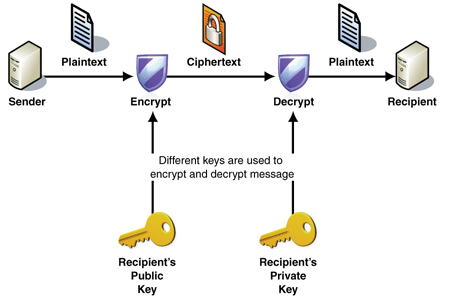
\includegraphics[scale=0.9]{graphics/HTTPS.png}
		\caption{HTTPS \cite{https_pic}.}
		\label{fig:HTTPS}
	\end{center} 
\end{figure}

\Cref{fig:HTTPS} shows how HTTPS works after the key exchange have taken place. First the sender sends plain text, which is encrypted using the recipients public key. The encrypted message is then send and decrypted using the recipients private key before plain text is received.

The handshake between the browser and a site using HTTPS starts with an exchange of public SSL-keys (Secure Socket Layer). The SSL-key is unique and enable encrypt of the data you send, the encrypted data can then only be decrypted with your own private key\cite{HTTPS}. 

\subsection*{Hashing}
Hash function are most commonly used to store a users password or other sensitive data. In functions as a one way function, when a message is hashed it can not be reversed again. The formal definition is shown below:
\begin{quote}
\textit{'A hash function is a computationally efficient function mapping binary strings of arbitrary length to binary strings of some fixed length, called hash-values.'\cite{Hash_def}}
\end{quote}

It have been requested by the heatmap application group to have a unique identification of all people. If we are not allowed to store the MAC-Address, a solution to this would be to hash the MAC-Address with a random, daily changing salt. In this way it will be possible for the heatmap to track people for as long af the salt-value is unchanged.

Java have a hash-method implemented in the object class called \textit{hashCode()}, this may be used for hashing information. When using a hash function properly, you add a random generated string that extends the original message. The generated string is called a salt and make the hash function more secure. An example of how to apply the Java hashCode can be seen in \cref{lst:hash}.
\begin{lstlisting}[caption={Hash a MAC-Address},label={lst:hash},language=inc_Java]
String salt = UUID.randomUUID().toString();
hash = MAC_Address + salt;
hash.hashCode();
\end{lstlisting}
In \cref{lst:hash} we see that a random string is generated in line one, then concatenated with the information we wish to hash, in this case the MAC-Address. Finally we call the Java hashCode() on the string, and this gives us a string that can not be traced back to the original.

\subsection*{Hard-coded passwords}
In our connection to Cisco as well as to the intermediate server we are currently using hard-coded passwords, which means that everyone with access to the code can find the log-in information. These should be hashed and stored such that the log-in can not be seen in the code and is never written as plain text. 

\subsection*{Visibility}
As of now the most of our system is public, by decreasing the level of visibility to have more private and protected classes and methods, the system would be more secure.
 
\subsection*{Obfuscate personal information}
In order to ensure our users personal information, it have been considered to obfuscate their E-mail as well as their Ip-addresses in the same manner as it is done to the MAC-address. By doing so there will be no way for outsiders to identify people unwilling to have their information stored.
